\subsection{The Cubic Fixed-Point Equation (CFE)}
%-----------------------------------------------------------------------------

\begin{definition}{Effective Potential Parameters}{params}
From the 11D Chern--Simons reduction (A5) and modulus-closure structure (A6):
\begin{align}
    A &= 2\cthree^3 = \frac{1}{256\pi^3} \approx 1.2598 \times 10^{-4}\\[0.5em]
    \mathcal{K} &= \frac{\bone}{2\pi}\ln\frac{1}{\phiz} \approx 1.9147
\end{align}
\textbf{Notation:} We use $\mathcal{K}$ (calligraphic) for this CFE parameter to 
distinguish it from $\kappa^2 = 8\pi G$ (gravitational coupling) and the contorsion tensor $K$.
\end{definition}

\begin{tcolorbox}[colback=gray!5, colframe=gray!60,
    title={\textbf{Lemma (Geometric Fixing of the Log)}}, fonttitle=\bfseries\small]
In TFPT the one-loop logarithm is the ratio of a UV scale to a geometrically fixed IR scale:
\begin{equation}
    \ln\frac{1}{\phiz} = \ln\frac{\Lambda}{\mu_{\text{geo}}}.
\end{equation}
Here $\mu_{\text{geo}} \equiv \ell_{\text{geo}}^{-1}$ is fixed by the M\"obius curvature
normalization ($R_{\text{total}}=6\pi$), and $\phiz = \ell_{\text{UV}}/\ell_{\text{geo}}$.
Thus the renormalization point is not a free choice but is geometrically determined.
\end{tcolorbox}

\begin{tcolorbox}[colback=yellow!3, colframe=yellow!60!black,
    title={\textbf{Quantization and scheme declaration}}, fonttitle=\bfseries\small]
\textbf{Scheme:} dimensional regularization, background-field gauge, $\overline{\mathrm{MS}}$.
\textbf{Coefficient policy:} we postulate the fixed coefficients in
$U(\alpha)=\frac{A}{4}\alpha^4-\frac{2}{3}A\cthree^3\alpha^3-8A\bone\cthree^6 L\,\alpha+\ldots$
within the declared scheme.
\textbf{Status:} postulated input, audited for internal consistency across suite implementations;
a full background-field derivation is deferred.
\end{tcolorbox}

\begin{tcolorbox}[colback=yellow!5, colframe=yellow!60!black,
    title={\textbf{Status of the $\alpha^2$ term and renorm condition}}, fonttitle=\bfseries\small]
\textbf{EFT framing:} $U(\alpha)$ is an EFT ansatz.
\textbf{Toy one-loop finding:} a quadratic term in $\alpha$ appears generically in the toy one-loop determinant.
\textbf{Renorm policy:} $\alpha^2$ term fixed by renormalization condition; we fix a counterterm $\delta c_2=-c_2$ at a declared reference point,
so the stationarity polynomial has no residual $\alpha^2$ term in the chosen scheme.
\textbf{Precision constraint:} the robustness scan requires $|\epsilon_2|\lesssim 1.58\times 10^{-10}$ to stay within 1 ppm.
\textbf{Toy scope:} toy model demonstration only; the toy $\beta$-prefactor mismatch is flagged and is not a Standard Model one-loop derivation.
\textbf{Evidence:} \texttt{alpha2\_renorm\_condition\_audit}, \texttt{alpha2\_term\_robustness\_scan}.
\textbf{Policy statement:} the absence of $\alpha^2$ is a renormalization condition, not a Ward-identity theorem.
\end{tcolorbox}

\begin{figure}[H]
\centering
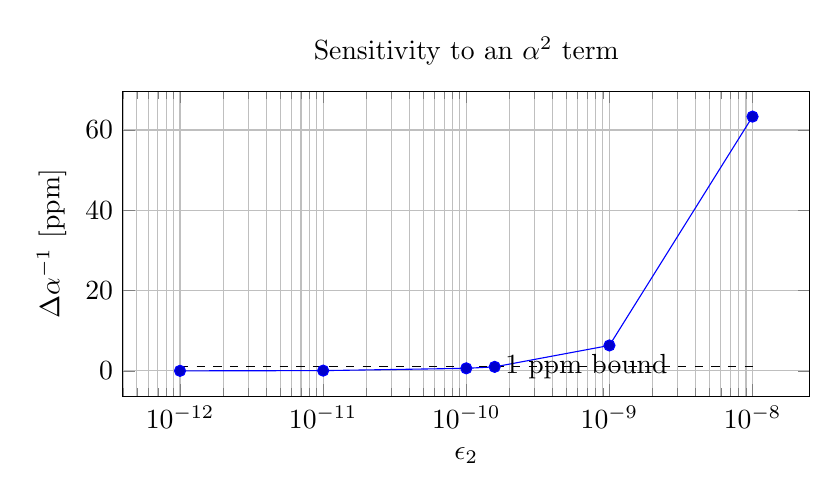
\begin{tikzpicture}
\begin{axis}[
  width=0.85\linewidth,
  height=0.45\linewidth,
  grid=both,
  xlabel={$\epsilon_2$},
  ylabel={$\Delta \alpha^{-1}$ [ppm]},
  xmode=log,
  title={Sensitivity to an $\alpha^2$ term},
]
\addplot table[row sep=\\] {
eps ppm\\
1e-12 0.006332528061424504\\
1e-11 0.06332528424435171\\
1e-10 0.6332532054543387\\
1.579153968e-10 1.0\\
1e-9 6.332568355779471\\
1e-8 63.32931383533495\\
};
\addplot[black, dashed] coordinates {(1e-12,1.0) (1e-8,1.0)};
\node[anchor=west] at (axis cs:1.6e-10,1.05) {1 ppm bound};
\end{axis}
\end{tikzpicture}
\caption{Robustness bound for a potential $\alpha^2$ contribution under the declared renormalization condition.}
\label{fig:alpha2-sensitivity}
\end{figure}

\begin{tcolorbox}[colback=yellow!5, colframe=yellow!60!black,
    title={\textbf{Scheme shifts and counterterm compensation}}, fonttitle=\bfseries\small]
\textbf{Raw drift:} a small shift $\delta L$ in the logarithm produces an order-$10^2$ ppm drift in $\alpha$.
\textbf{Compensation:} a local counterterm $\delta U = C_{\mathrm{ct}}\,\alpha$ cancels the shift,
and the compensated residuals are numerically zero ($\sim 10^{-56}$ ppm) across $\delta L\in[-0.005,0.005]$.
\textbf{No fit freedom:} $C_{\mathrm{ct}}$ is fixed by the declared scheme choice, not by data fitting.
\textbf{Evidence:} \texttt{scheme\_shift\_sensitivity\_audit}, \texttt{scheme\_shift\_compensated\_invariance\_audit}.
\end{tcolorbox}

\begin{figure}[H]
\centering
\begin{tikzpicture}
\begin{groupplot}[
  group style={group size=2 by 1, horizontal sep=1.0cm},
  width=0.48\linewidth,
  height=0.40\linewidth,
  grid=both,
]
\nextgroupplot[
  title={Scheme shift sensitivity (raw)},
  xlabel={$\delta L$},
  ylabel={$\Delta \alpha^{-1}$ [ppm]},
]
\addplot coordinates {
  (-0.001, 112.96609230847633)
  (-0.0005, 56.47664727232789)
  (0.0, 0.0)
  (0.0005, -56.46385458573416)
  (0.001, -112.91492155922317)
};

\nextgroupplot[
  title={Scheme shift compensated},
  xlabel={$\delta L$},
  ylabel={residual [ppm]},
]
\addplot coordinates {
  (-0.005, 3.5424860278915774e-56)
  (-0.001, 4.630145519251477e-56)
  (0.0, 3.218820203992068e-56)
  (0.001, 5.026307150589819e-56)
  (0.005, 2.8951464379576505e-56)
};
\end{groupplot}
\end{tikzpicture}
\caption{Scheme shift sensitivity and counterterm compensation.}
\label{fig:scheme-shift}
\end{figure}

\begin{theorem}{Cubic Fixed-Point Equation}{CFE}
Adopting the minimal coefficient policy for $U(\alpha)$ in the declared scheme, the
vacuum extremum $\delta\Gamma_{\mathrm{eff}}/\delta\sigma=0$ is equivalent to
$\partial U/\partial\alpha = 0$ and yields the cubic fixed-point equation:
\begin{equation}
    \boxed{\alpha^3 - 2\cthree^3\,\alpha^2 - 8\bone\cthree^6\ln\frac{1}{\phiz(\alpha)} = 0}
    \label{eq:CFE}
\end{equation}
This equation has exactly one positive real root.
\end{theorem}

\begin{proof}
In the declared scheme we adopt the coefficient policy for the effective potential
\begin{equation}
    U(\alpha) = \frac{A}{4}\alpha^4 - \frac{2}{3}A\cthree^3\alpha^3 - 8A\bone\cthree^6 L\,\alpha + \ldots
\end{equation}
where $L = \ln(1/\phiz)$. The modulus-closure condition 
$\delta\Gamma_{\mathrm{eff}}/\delta\sigma = 0$ reduces to $\partial U/\partial\alpha = 0$
(monotonic $\alpha(\sigma)$), giving
\begin{equation}
    A\bigl[\alpha^3 - 2\cthree^3\alpha^2 - 8\bone\cthree^6 L\bigr] = 0
\end{equation}
(The factor 2 arises from differentiating the $2/3$ coefficient of the cubic term.)
For $A \neq 0$, this is the CFE. Descartes' rule of signs guarantees exactly 
one positive real root.
\end{proof}

\begin{figure}[H]
\centering
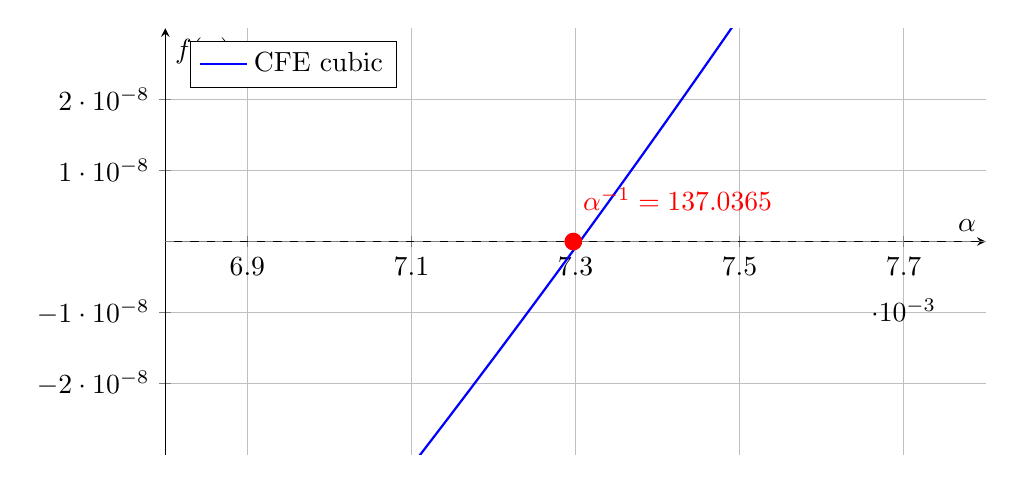
\begin{tikzpicture}
\begin{axis}[
    width=12cm, height=7cm,
    xlabel={$\alpha$},
    ylabel={$f(\alpha)$},
    xmin=0.0068, xmax=0.0078,
    ymin=-3e-8, ymax=3e-8,
    grid=major,
    axis lines=middle,
    xtick={0.0069, 0.0071, 0.0073, 0.0075, 0.0077},
    ytick={-2e-8, -1e-8, 0, 1e-8, 2e-8},
    scaled y ticks=false,
    yticklabel style={/pgf/number format/sci},
    legend pos=north west
]
    % CFE cubic
    \addplot[domain=0.0068:0.0078, samples=200, thick, blue] 
        {x^3 - 2*0.039788735773^3*x^2 - 8*4.1*0.039788735773^6*2.9439};
    \addlegendentry{CFE cubic}
    
    % Root marker
    \addplot[only marks, mark=*, mark size=3pt, red] 
        coordinates {(0.00729733, 0)};
    \node[red, above right] at (axis cs:0.00729733, 0.3e-8) 
        {$\alpha^{-1} = 137.0365$};
    
    % Zero line
    \addplot[domain=0.0068:0.0078, dashed, gray] {0};
\end{axis}
\end{tikzpicture}
\caption{The CFE has a unique positive root at $\alpha \approx 0.007297$, 
corresponding to $\alpha^{-1} \approx 137.0365$ (baseline with fixed $\phiz$).}
\label{fig:CFE}
\end{figure}

\begin{figure}[H]
\centering
\begin{tikzpicture}
\begin{groupplot}[
    group style={group size=2 by 1, horizontal sep=1.2cm},
    width=0.45\linewidth,
    height=0.36\linewidth
]
\pgfmathsetmacro{\cThree}{0.039788735772973834}
\pgfmathsetmacro{\CfeC}{3.818809423599759e-7}
\pgfmathsetmacro{\alphaRoot}{0.007297325816919221}
\pgfmathsetmacro{\alphaStar}{8.3988370919790336e-5}
\pgfmathsetmacro{\fAlphaStar}{-3.818812385889108e-7}

\nextgroupplot[
    xlabel={$\alpha$},
    ylabel={$f(\alpha)$},
    grid=major
]
\addplot[domain=0:0.02, samples=400, thick] {x^3 - 2*(\cThree^3)*x^2 - \CfeC};
\addplot[black, dashed] coordinates {(0,0) (0.02,0)};
\addplot[only marks, mark=*, mark size=2.5pt] coordinates {(\alphaRoot,0)};
\addlegendentry{root (baseline)}
\addplot[only marks, mark=square*, mark size=2.5pt] coordinates {(\alphaStar,\fAlphaStar)};
\addlegendentry{$\alpha_\ast$ (local min)}

\nextgroupplot[
    xlabel={fixed-point iteration},
    ylabel={$|\Delta\alpha|$},
    ymode=log,
    grid=major
]
\addplot+[mark=o] coordinates {
    (0,2.7017585695945706e-08)
    (1,9.9302866397459317e-14)
    (2,3.6498668384968009e-19)
    (3,1.3415048751400539e-24)
    (4,4.9306876378145135e-30)
    (5,1.8122692680605213e-35)
};
\end{groupplot}
\end{tikzpicture}
\caption{CFE uniqueness certificate (suite). Left: baseline cubic with unique root. Right: fixed-point iteration convergence.}
\label{fig:cfe-unique-suite}
\end{figure}

\begin{figure}[H]
\centering
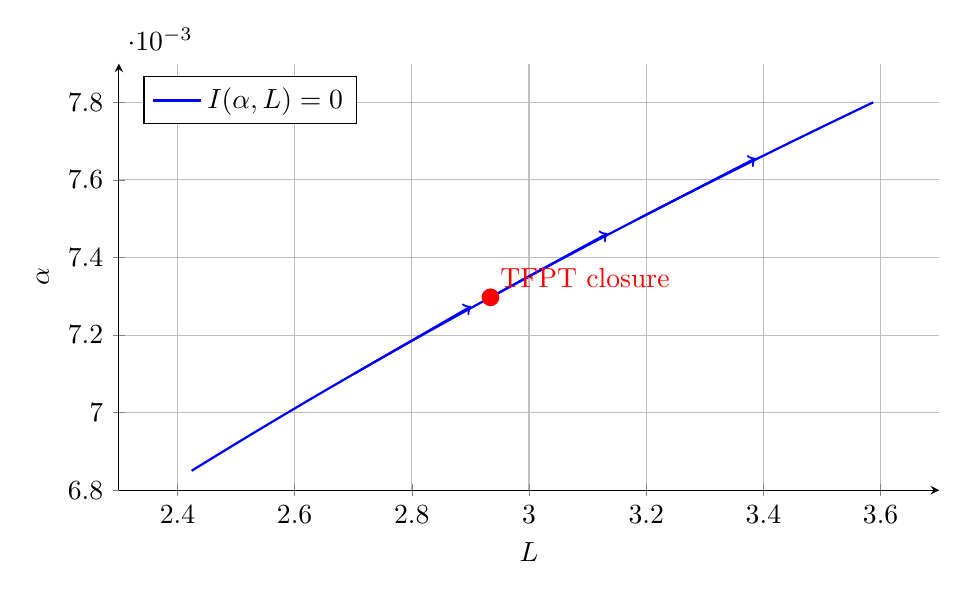
\begin{tikzpicture}
\begin{axis}[
    width=12cm, height=7cm,
    xlabel={$L$},
    ylabel={$\alpha$},
    xmin=2.3, xmax=3.7,
    ymin=0.0068, ymax=0.0079,
    grid=major,
    axis lines=left,
    legend pos=north west
]
    % Invariant surface I(\alpha,L)=0 (parametric form L(\alpha),\alpha)
    \addplot[domain=0.00685:0.0078, samples=240, thick, blue]
        ({(x^3 - 2*0.039788735773^3*x^2)/(8*4.1*0.039788735773^6)}, {x});
    \addlegendentry{$I(\alpha,L)=0$}

    % Flow direction from implicit differentiation: d\alpha/dL
    \addplot[->, thick, blue] coordinates {(2.701252,0.00710000) (2.901252,0.00727418)};
    \addplot[->, thick, blue] coordinates {(2.934229,0.00729733) (3.134229,0.00746216)};
    \addplot[->, thick, blue] coordinates {(3.187073,0.00750000) (3.387073,0.00765600)};

    % TFPT closure point (baseline)
    \addplot[only marks, mark=*, mark size=3pt, red] coordinates {(2.934224,0.00729733)};
    \node[red, above right] at (axis cs:2.934224,0.00729733) {TFPT closure};
\end{axis}
\end{tikzpicture}
\caption{Structural flow on the invariant surface $I(\alpha,L)=0$ in the $(L,\alpha)$ plane,
with arrows indicating $d\alpha/dL$ from implicit differentiation.
The marked point shows the TFPT closure solution.}
\label{fig:invariant_flow}
\end{figure}

%-----------------------------------------------------------------------------
\subsection{Geometric Self-Consistency (Backreaction)}
%-----------------------------------------------------------------------------

\subsubsection{Backreaction as Structural Response}

The response $\phiz(\alpha) = \phitree + \deltatop e^{-2\alpha}$ is the closed form
consequence of defect sector reweighting on the orientable double cover. The linear form
is the $\mathcal{O}(\alpha)$ expansion, not a separate assumption.

\textbf{Step 1: The CFE uses $L = \ln(1/\phiz)$ as input.}
The cubic fixed-point equation \eqref{eq:CFE} depends on $\phiz$ only through 
the logarithm $L$. Any shift in $\phiz$ propagates via:
\begin{equation}
    \delta L = -\frac{\delta\phiz}{\phiz}
\end{equation}

\textbf{Step 2: Defect sector reweighting in the Euclidean partition function.}
We treat the discrete correction as a defect sector weight. An additive deformation of the
defect action by $\alpha$ implies exact exponential reweighting:
\begin{lemma}{Defect Sector Reweighting}{defectreweight}
Let the Euclidean partition function split into sectors
\begin{equation}
    Z(\alpha)=Z_{\mathrm{triv}}(\alpha)+Z_{\mathrm{def}}(\alpha),
\end{equation}
with defect weight $\delta_{\mathrm{top}}(\alpha)=Z_{\mathrm{def}}(\alpha)/Z_{\mathrm{triv}}(\alpha)$.
If the defect action is deformed additively,
\begin{equation}
    S_{\mathrm{def}}(\alpha)=S_{\mathrm{def}}(0)+\alpha\,\mathcal{J},
\end{equation}
then
\begin{equation}
    \delta_{\mathrm{top}}(\alpha)=\delta_{\mathrm{top}}\,e^{-\alpha\mathcal{J}}.
\end{equation}
For a degree-$d$ cover with identical sheet contributions, $\mathcal{J}=d\,\mathcal{J}_1$.
We identify the per-sheet normalization with the spectral-flow unit, $\mathcal{J}_1=\mathrm{SF}$,
so $\mathcal{J}=d\,\mathrm{SF}$. For the orientable double cover, $d=2$ and $\mathrm{SF}=1$,
so the exponent is fixed to $k=2$ and
$\delta_{\mathrm{top}}(\alpha)=\delta_{\mathrm{top}}\,e^{-2\alpha}$. If $\mathrm{SF}\neq 1$,
this corresponds to a different topological sector with a different $k$. \hfill QED
\end{lemma}
\textbf{Evidence:} \texttt{backreaction\_index\_anchor\_audit}.

\begin{tcolorbox}[colback=blue!3, colframe=blue!40, 
    title={\textbf{Lemma (Cover-Degree Scaling of Deck-Invariant Response)}}, fonttitle=\bfseries\small]
Let $p:\widetilde{M}\to M$ be a degree-$d$ covering and let $\mathcal{J}$ be a deck-invariant
source functional. Then
\begin{equation}
    \int_{\widetilde{M}}\mathcal{J} = d \int_{M}\mathcal{J}.
\end{equation}
If the response of $\phiz$ is built from such an integrated source, the effective
weight acquires a factor $d$. For the orientable double cover, $d=2$.
\end{tcolorbox}

\textbf{Step 3: Double cover fixes the exponent.}
The defect-sector lemma and cover-degree scaling fix the exponent to $2$ for the
orientable double cover. Adding the baseline yields the exact response:
\begin{equation}
    \phiz(\alpha) = \phitree + \deltatop\,e^{-2\alpha}.
\end{equation}

\begin{remark}
\textbf{Series control (no new parameters):} The exact form implies
\begin{equation}
    \phiz(\alpha)=\phitree+\deltatop\left(1-2\alpha+2\alpha^2-\frac{4}{3}\alpha^3+\cdots\right),
\end{equation}
so all higher coefficients are fixed (e.g.\ $c_2=2$). Numerically, even the
$\alpha^2$ term shifts $\phiz$ by $\lesssim 10^{-8}$ since
$\alpha\approx 0.0073$ and $\deltatop\approx 1.2\times10^{-4}$.
\end{remark}

\begin{theorem}{Self-Consistent $\alpha$ with Derived Two-Defect Partition}{selfconsistent}
Including the minimal backreaction response on the orientable double cover \emph{and} the derived two-defect occupancy weight anchored by holonomy degeneracy $g=5$:
\begin{align}
    \phiz(\alpha) &= \phitree + \deltatop e^{-2\alpha} + \delta_2 e^{-4\alpha} + \cdots,
    \label{eq:backreaction}\\
    \delta_2 &= \frac{g}{4}\,(\delta_{\mathrm{top}})^2 = \frac54\,(\delta_{\mathrm{top}})^2,
    \qquad (g=5),
\end{align}
where $g$ is fixed by SU(5) holonomy degeneracy prior to any $\alpha$ comparison (see theoryv3 audit chain).
The prefactor $g/4$ follows from the two-defect cluster expansion with the pair symmetry
factor $1/2$ and the two-sheet pairing factor $2$ (Appendix~\ref{app:repro}).
\textbf{Evidence:} \texttt{two\_defect\_cluster\_expansion\_audit}, \texttt{g5\_independence\_audit}, \texttt{g5\_trace\_completeness\_audit}.
the self-consistent solution of the CFE yields the v2.7 headline value:
\begin{equation}
    \boxed{\alpha^{-1}_{\text{TFPT}}(0) = \num[round-mode=places,round-precision=12]{\TFPTalphaInvGOverFourNum}}
\end{equation}
with CODATA 2022 diagnostic $z=\num[round-mode=places,round-precision=3]{\TFPTalphaZGOverFourNum}$ (see theoryv3 module \texttt{defect\_partition\_g5\_audit}; artifacts in Appendix~\ref{app:repro}).
\end{theorem}

\begin{lemma}{One-defect truncation (diagnostic baseline; excluded at CODATA precision)}{oneDefectTruncation}
Setting $\delta_2=0$ in \eqref{eq:backreaction} yields the one-defect truncation
\[
\alpha^{-1}(0)=\num[round-mode=places,round-precision=10]{\TFPTalphaInvSelfNum},
\]
which is useful as an expansion baseline and for sensitivity plots, but is not the headline prediction.
\end{lemma}

\begin{remark}
\textbf{Diagnostic-only templates:} legacy $g$ variants (e.g.\ the ordered-occupancy $g=4$ case) are
recorded as internal sanity checks in Appendix~\ref{app:gdiagnostic} and are not used for
parameter selection.
\end{remark}

\begin{proof}
On the orientable double cover $\widetilde{M}$, defect-sector reweighting with a
deck-invariant source fixes the exponent in \eqref{eq:backreaction}
(Lemma~\ref{lem:defectreweight}). The self-consistent solution is obtained by iteration:
\begin{enumerate}
    \item Start with $\alpha_0$ from the CFE with fixed $\phiz$.
    \item Update $\phiz(\alpha_n)$ via \eqref{eq:backreaction}.
    \item Solve CFE for $\alpha_{n+1}$.
    \item Iterate until convergence.
\end{enumerate}
Convergence is rapid (typically 3--4 iterations).
\end{proof}

\begin{table}[H]
\centering
\small
\setlength{\tabcolsep}{4pt}
\begin{tabularx}{\linewidth}{@{}lccX@{}}
\toprule
\textbf{Scenario} & $\alpha^{-1}$ & \textbf{Deviation from CODATA} & \textbf{Status}\\
\midrule
Baseline (fixed $\phiz$) & 137.03650146 & $+3.67$ ppm & structural\\
Self-consistent $\phiz(\alpha)$ & \num[round-mode=places,round-precision=10]{\TFPTalphaInvSelfNum} & $-0.037$ ppm & \textbf{closed-form defect reweighting (one-defect)}\\
Two-defect refinement ($+\tfrac54(\deltatop)^2 e^{-4\alpha}$) & \num[round-mode=places,round-precision=12]{\TFPTalphaInvGOverFourNum} & $+\num[round-mode=places,round-precision=6]{\TFPTalphaPpmGOverFourNum}$ ppm & \textbf{derived (holonomy $g=5$)}\\
Two-defect (suite diagnostic) ($+(\deltatop)^2 e^{-4\alpha}$) & \num[round-mode=places,round-precision=10]{\TFPTalphaInvTwoDefNum} & $\num[round-mode=places,round-precision=4]{\TFPTalphaPpmTwoDefNum}$ ppm & parameter-free template (diagnostic)\\
CODATA 2022 & \num[round-mode=places,round-precision=9]{\TFPTalphaInvCODATANum} & --- & reference\\
\bottomrule
\end{tabularx}
\caption{Impact of geometric self-consistency on $\alpha$ prediction.}
\label{tab:alpha}
\end{table}

% Suite/theoryv3 audit table for α
\TFPTAlphaAuditTable

